% Generated by pysimcount.figleader -- do not edit; regenerate instead.
% figure: main-t-all-formulas -- cost at n = 500, one row per formula
% seeds [1, 2, 3, 4, 5, 6, 7, 8, 9, 10]; metric=t kind=xyz merged (Clifford+T (ct), simcount template)
% shown: suzuki4, suzuki6, mo-q6, mo-q14, bm-q10, mo-o8-q21, morales-y8m10, morales-m8
% removed (see main-t-all-formulas-ranking.md): lie-trotter, suzuki2, suzuki8
% n = 500; x = the source record's plotted value; bars min..max over seeds
% cheapest on = seeds on which the formula is cheapest; rank range = min..max of its rank over seeds
% per-seed values: runs' totals if measured, else each seed's own fit c(n) ceil(a_s n^b_s)
% row order (plotted value) and mean-rank order agree
% derived: main-t-all-formulas.json by pysimcount.figleader; source_sha256=e2b784407e82d3de3175dfa318f56f47f0de675e8adb0038f54747cd6140373b
% figure made at git_commit=eed0c490bd2a7ed3c821acf76ae930c79d2195f6 git_dirty=False
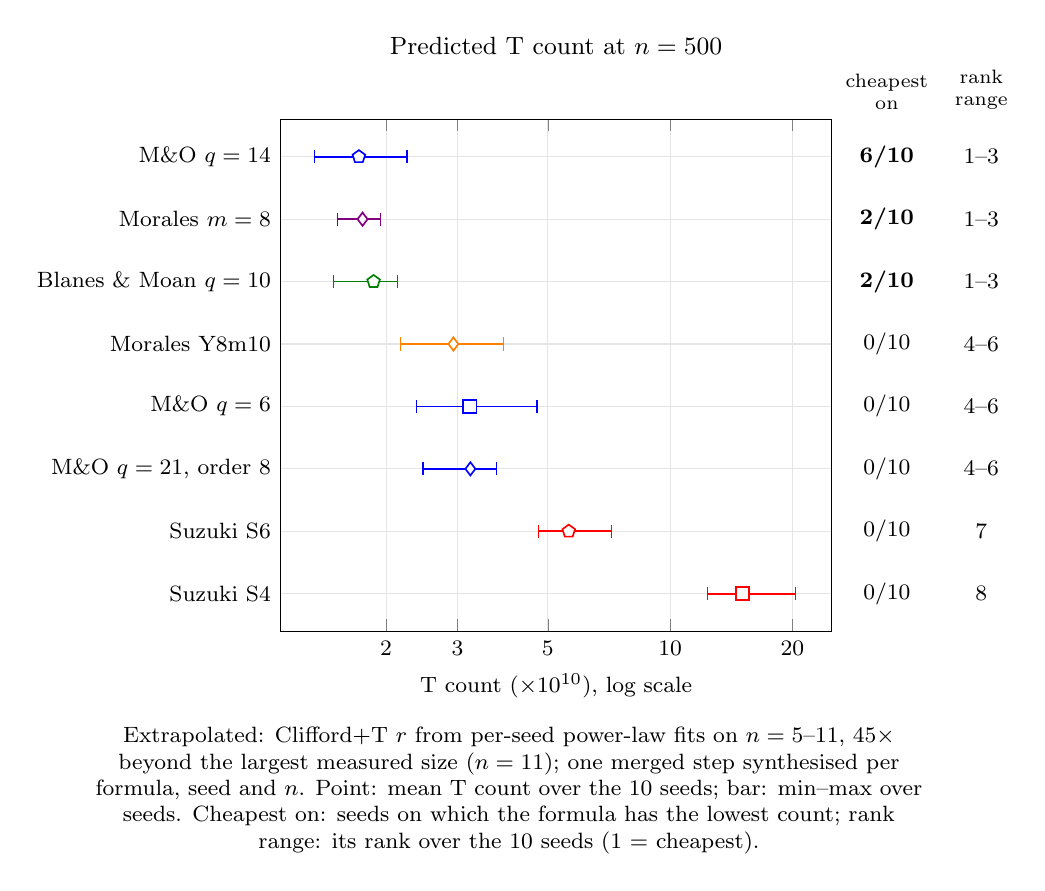
\begin{tikzpicture}
  \begin{semilogxaxis}[
    scale only axis, clip=false,
    at={(0cm,0cm)}, anchor=south west,
    width=7.0cm, height=6.5cm,
    title={Predicted T count at $n = 500$}, title style={font=\small, yshift=14pt},
    xlabel={T count ($\times 10^{10}$), log scale}, xlabel style={font=\footnotesize},
    xmin=1.1e+10, xmax=2.5e+11, xtick={2e+10,3e+10,5e+10,1e+11,2e+11}, xticklabels={2,3,5,10,20},
    xminorticks=false,
    y dir=reverse, ymin=0.4, ymax=8.6, ytick={1,2,3,4,5,6,7,8},
    yticklabels={{M\&O $q=14$},{Morales $m=8$},{Blanes \& Moan $q=10$},{Morales Y8m10},{M\&O $q=6$},{M\&O $q=21$, order 8},{Suzuki S6},{Suzuki S4}},
    tick label style={font=\footnotesize}, ytick style={draw=none},
    xmajorgrids=true, ymajorgrids=true, grid style={black!10},
  ]
    % mo-q14: plotted 1.71426e+10, seeds 1.33055e+10..2.2523e+10, cheapest on 6/10, rank 1..3
    \addplot[blue, only marks, mark=pentagon*, mark size=2.4pt, mark options={solid, fill=white, line width=0.6pt}, error bars/.cd, x dir=both, x explicit, error bar style={solid, line width=0.6pt}] coordinates {
      (1.71426e+10,1) += (5.38038e+09,0) -= (3.83706e+09,0)
    };
    % morales-m8: plotted 1.75035e+10, seeds 1.51658e+10..1.94095e+10, cheapest on 2/10, rank 1..3
    \addplot[violet, only marks, mark=diamond*, mark size=2.4pt, mark options={solid, fill=white, line width=0.6pt}, error bars/.cd, x dir=both, x explicit, error bar style={solid, line width=0.6pt}] coordinates {
      (1.75035e+10,2) += (1.90596e+09,0) -= (2.33772e+09,0)
    };
    % bm-q10: plotted 1.86331e+10, seeds 1.48173e+10..2.13136e+10, cheapest on 2/10, rank 1..3
    \addplot[green!50!black, only marks, mark=pentagon*, mark size=2.4pt, mark options={solid, fill=white, line width=0.6pt}, error bars/.cd, x dir=both, x explicit, error bar style={solid, line width=0.6pt}] coordinates {
      (1.86331e+10,3) += (2.68049e+09,0) -= (3.81581e+09,0)
    };
    % morales-y8m10: plotted 2.92891e+10, seeds 2.17099e+10..3.88229e+10, cheapest on 0/10, rank 4..6
    \addplot[orange, only marks, mark=diamond*, mark size=2.4pt, mark options={solid, fill=white, line width=0.6pt}, error bars/.cd, x dir=both, x explicit, error bar style={solid, line width=0.6pt}] coordinates {
      (2.92891e+10,4) += (9.53382e+09,0) -= (7.5792e+09,0)
    };
    % mo-q6: plotted 3.21589e+10, seeds 2.37233e+10..4.7055e+10, cheapest on 0/10, rank 4..6
    \addplot[blue, only marks, mark=square*, mark size=2.4pt, mark options={solid, fill=white, line width=0.6pt}, error bars/.cd, x dir=both, x explicit, error bar style={solid, line width=0.6pt}] coordinates {
      (3.21589e+10,5) += (1.48961e+10,0) -= (8.4356e+09,0)
    };
    % mo-o8-q21: plotted 3.22461e+10, seeds 2.46524e+10..3.74206e+10, cheapest on 0/10, rank 4..6
    \addplot[blue, only marks, mark=diamond*, mark size=2.4pt, mark options={solid, fill=white, line width=0.6pt}, error bars/.cd, x dir=both, x explicit, error bar style={solid, line width=0.6pt}] coordinates {
      (3.22461e+10,6) += (5.17455e+09,0) -= (7.59363e+09,0)
    };
    % suzuki6: plotted 5.631e+10, seeds 4.74716e+10..7.17507e+10, cheapest on 0/10, rank 7..7
    \addplot[red, only marks, mark=pentagon*, mark size=2.4pt, mark options={solid, fill=white, line width=0.6pt}, error bars/.cd, x dir=both, x explicit, error bar style={solid, line width=0.6pt}] coordinates {
      (5.631e+10,7) += (1.54407e+10,0) -= (8.83844e+09,0)
    };
    % suzuki4: plotted 1.5088e+11, seeds 1.23785e+11..2.03957e+11, cheapest on 0/10, rank 8..8
    \addplot[red, only marks, mark=square*, mark size=2.4pt, mark options={solid, fill=white, line width=0.6pt}, error bars/.cd, x dir=both, x explicit, error bar style={solid, line width=0.6pt}] coordinates {
      (1.5088e+11,8) += (5.3077e+10,0) -= (2.70956e+10,0)
    };
    \node[anchor=south, font=\scriptsize, align=center] at ([xshift=0.7cm]axis cs:2.5e+11,0.4) {cheapest\\on};
    \node[anchor=south, font=\scriptsize, align=center] at ([xshift=1.9cm]axis cs:2.5e+11,0.4) {rank\\range};
    \node[font=\footnotesize\bfseries] at ([xshift=0.7cm]axis cs:2.5e+11,1) {6/10};
    \node[font=\footnotesize] at ([xshift=1.9cm]axis cs:2.5e+11,1) {1--3};
    \node[font=\footnotesize\bfseries] at ([xshift=0.7cm]axis cs:2.5e+11,2) {2/10};
    \node[font=\footnotesize] at ([xshift=1.9cm]axis cs:2.5e+11,2) {1--3};
    \node[font=\footnotesize\bfseries] at ([xshift=0.7cm]axis cs:2.5e+11,3) {2/10};
    \node[font=\footnotesize] at ([xshift=1.9cm]axis cs:2.5e+11,3) {1--3};
    \node[font=\footnotesize] at ([xshift=0.7cm]axis cs:2.5e+11,4) {0/10};
    \node[font=\footnotesize] at ([xshift=1.9cm]axis cs:2.5e+11,4) {4--6};
    \node[font=\footnotesize] at ([xshift=0.7cm]axis cs:2.5e+11,5) {0/10};
    \node[font=\footnotesize] at ([xshift=1.9cm]axis cs:2.5e+11,5) {4--6};
    \node[font=\footnotesize] at ([xshift=0.7cm]axis cs:2.5e+11,6) {0/10};
    \node[font=\footnotesize] at ([xshift=1.9cm]axis cs:2.5e+11,6) {4--6};
    \node[font=\footnotesize] at ([xshift=0.7cm]axis cs:2.5e+11,7) {0/10};
    \node[font=\footnotesize] at ([xshift=1.9cm]axis cs:2.5e+11,7) {7};
    \node[font=\footnotesize] at ([xshift=0.7cm]axis cs:2.5e+11,8) {0/10};
    \node[font=\footnotesize] at ([xshift=1.9cm]axis cs:2.5e+11,8) {8};
  \end{semilogxaxis}
  \node[anchor=north, text width=10.5cm, align=flush center, font=\footnotesize] at (2.9cm,-1.1cm) {Extrapolated: Clifford+T $r$ from per-seed power-law fits on $n = 5$--$11$, 45$\times$ beyond the largest measured size ($n = 11$); one merged step synthesised per formula, seed and $n$. Point: mean T count over the 10 seeds; bar: min--max over seeds. Cheapest on: seeds on which the formula has the lowest count; rank range: its rank over the 10 seeds (1 = cheapest).};
\end{tikzpicture}
